% Digital Logic Report Template
% Created: 2020-01-10, John Miller

%==========================================================
%=========== Document Setup  ==============================

% Formatting defined by class file
\documentclass[11pt]{article}

% ---- Document formatting ----
\usepackage[margin=1in]{geometry}	% Narrower margins
\usepackage{booktabs}				% Nice formatting of tables
\usepackage{graphicx}				% Ability to include graphics

%\setlength\parindent{0pt}	% Do not indent first line of paragraphs 
\usepackage[parfill]{parskip}		% Line space b/w paragraphs
%	parfill option prevents last line of pgrph from being fully justified

% Parskip package adds too much space around titles, fix with this
\RequirePackage{titlesec}
\titlespacing\section{0pt}{8pt plus 4pt minus 2pt}{3pt plus 2pt minus 2pt}
\titlespacing\subsection{0pt}{4pt plus 4pt minus 2pt}{-2pt plus 2pt minus 2pt}
\titlespacing\subsubsection{0pt}{2pt plus 4pt minus 2pt}{-6pt plus 2pt minus 2pt}

% ---- Hyperlinks ----
\usepackage[colorlinks=true,urlcolor=blue]{hyperref}	% For URL's. Automatically links internal references.

% ---- Code listings ----
\usepackage{listings} 					% Nice code layout and inclusion
\usepackage[usenames,dvipsnames]{xcolor}	% Colors (needs to be defined before using colors)

% Define custom colors for listings
\definecolor{listinggray}{gray}{0.98}		% Listings background color
\definecolor{rulegray}{gray}{0.7}			% Listings rule/frame color

% Style for Verilog
\lstdefinestyle{Verilog}{
	language=Verilog,					% Verilog
	backgroundcolor=\color{listinggray},	% light gray background
	rulecolor=\color{blue}, 			% blue frame lines
	frame=tb,							% lines above & below
	linewidth=\columnwidth, 			% set line width
	basicstyle=\small\ttfamily,	% basic font style that is used for the code	
	breaklines=true, 					% allow breaking across columns/pages
	tabsize=3,							% set tab size
	commentstyle=\color{gray},	% comments in italic 
	stringstyle=\upshape,				% strings are printed in normal font
	showspaces=false,					% don't underscore spaces
}

% How to use: \Verilog[listing_options]{file}
\newcommand{\Verilog}[2][]{%
	\lstinputlisting[style=Verilog,#1]{#2}
}




%======================================================
%=========== Body  ====================================
\begin{document}

\title{ELC 2137 Lab 04: Subtractor}
\author{Yiting Wang}

\maketitle


\section*{Summary}

	In this lab, it is to compare various implementations of a two-bit adder/subtractor. This is a relatively simple circuit that has sufficient complexity to high light some important aspects of digital circuit design. After completing this lab, I can describe the operation of a two-bit adder/sub-tractor, and develop a moderately complex circuit on abreadboard using standard electrical parts, develop my own test procedure and verify op-eration of the circuit, also I may can recognize that digital circuits quickly become complex and difficult to implement in hardware



\section*{Q\&A}

	\begin{enumerate}
		\item Why did we use two full adders instead of a half adder and a full adder?\\
			The main difference between a half-adder and a full-adder is that the full-adder has three inputs and two outputs. The first two inputs are A and B and the third input is an input carry designated as CIN. In here, we use two full adders instead of a half adder and a full adder, cause we need a third input to repersent the signed number.\\
			
		\item How many input combinations would it take to exhaustively test the adder/subtractor?\\
			16.\\
			
		\item Why were the combinations given in the truth table chosen?\\
			Cause we can use 3 for add and 3 for subtracte to figure out the rule for how the two-bit adder/subtractor works\\
		
		\item Do the results from your adder/subtractor match what you would expect from theory? Explain any discrepancies.\\
			The results are close to, but don’t exactly agree with the theory behind it. The MSB is different from what I expected. When the result should be a positive signed number, it shows negative; when the result should be a negative signed number, it shows positive.\\
		
	\end{enumerate}



\section*{Results}

	Figure 1 is the picture of my two bit adder/subtractor circuit, I built it based on the two bit adder/subtractor schematic. I only add 2 XOR gates for B 2's compliment in two bit adder.\\
	\begin{figure}[ht]\centering
		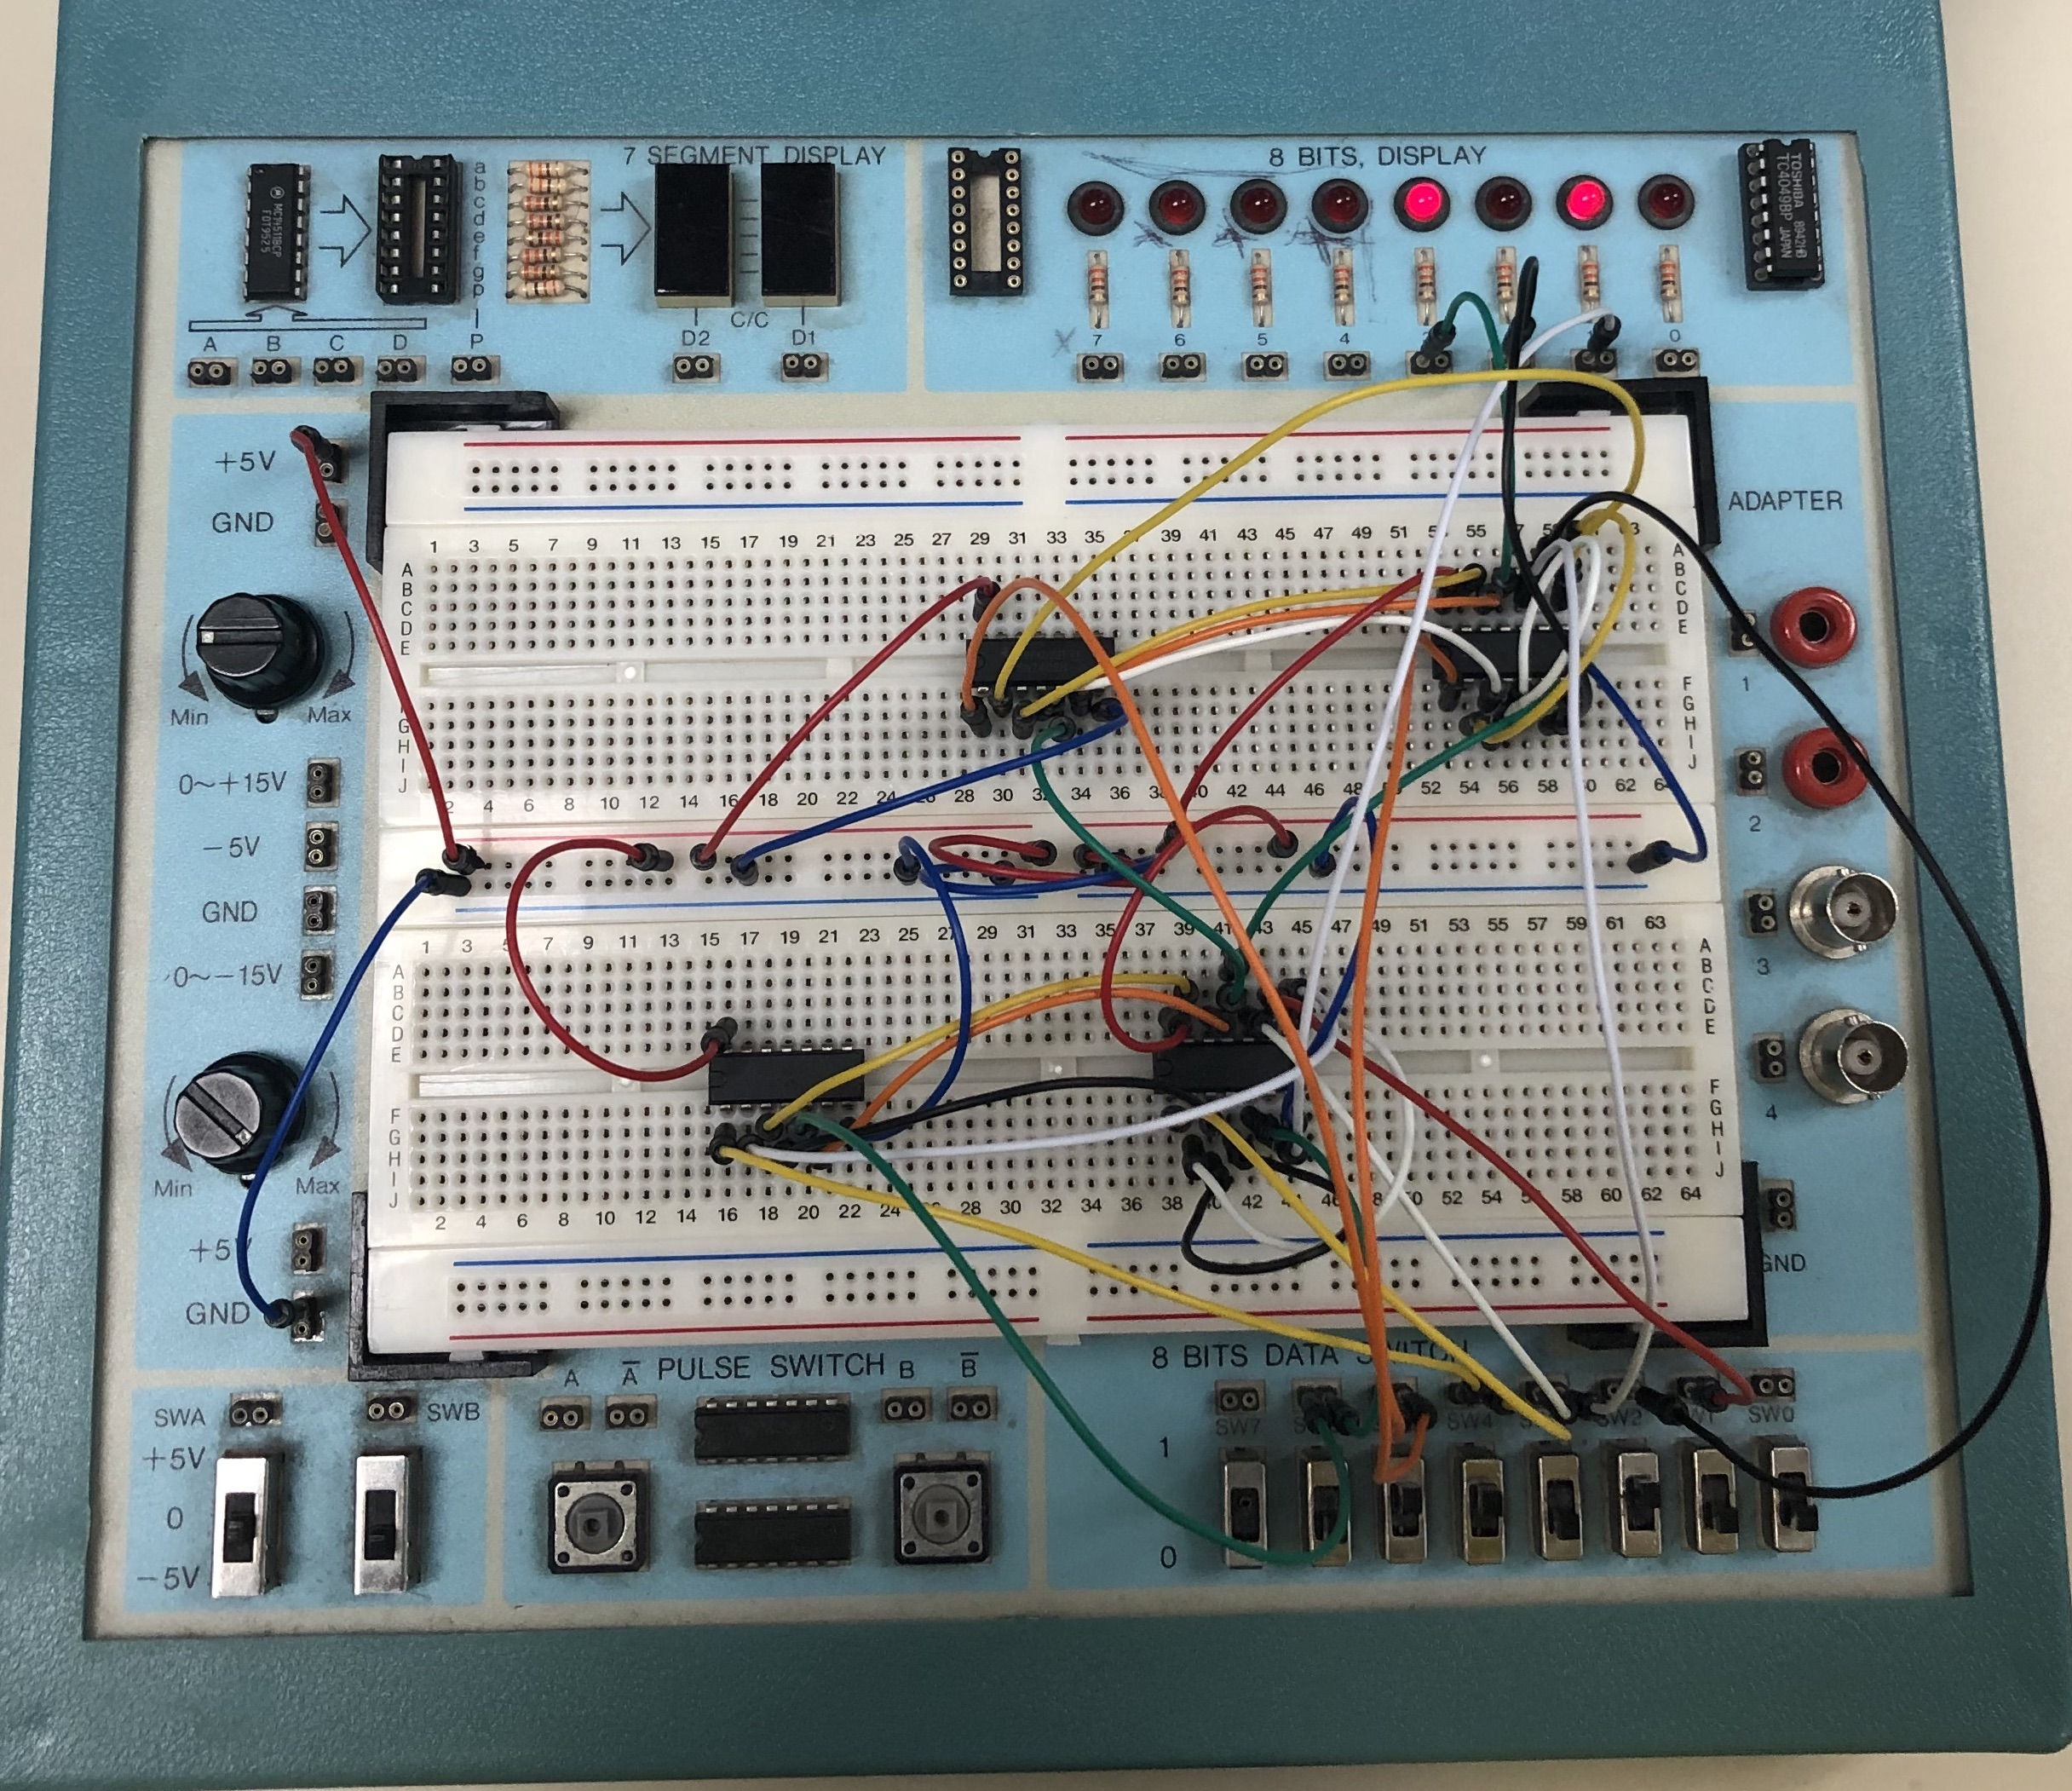
\includegraphics[width=0.7\textwidth,trim=5cm 5cm 5cm 5cm,clip]{2-bitSubtractor}
		\caption{The  two bit adder/subtractor Circuit}
		\label{fig:2-bitSubtractor}
	\end{figure}
	
	Figure 2 is the picture of my two-bit adder/subtractor schematic. I add 2 XOR gates for B 2's compliment before the B input in two bit adder.\\
	\begin{figure}[ht]\centering
		\includegraphics[width=1.0\textwidth]{Schematic}
		\caption{The two-bit adder/subtractor schematic}
		\label{fig:Schematic}
	\end{figure}
	
	Figure 3 is the cricuit domonstration page. It has the Expected Results Table and instructor signature.\\
	\begin{figure}[ht]\centering
		\includegraphics[width=1.0\textwidth]{Lab4Page}
		\caption{The cricuit domonstration page}
		\label{fig:Lab4Page}
	\end{figure}



\section*{Code}

	There is no code require in this lab.\\	



\end{document}
